\chapter{GameObject ``Player`` \& Komponenten}

Die Spielfigur, die der Anwender bedient stellte sich w"ahrend der Entwicklung als komplexestes GameObject heraus. In diesem Kapitel geben wir daher einen "Uberblick "uber die Realisierung mithilfe von Sprites sowie der verschiedenen anh"angenden und selbsterstellten Skripte

\begin{figure}
	\centering
	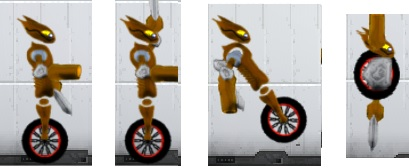
\includegraphics[height=5cm]{images/AnimationenZusammenschnitt.jpg}
	\caption{Zusammenschnitt der Player Sprites}
	\label{fig:playerSprites}
\end{figure}

\section{SpriteRenderer}

\section{AttributeComponent Skript}
Die AttributeComponent dient dazu die spielmechanischen Daten zu hinterlegen und zu verwalten. Sie kann sowohl dem Spieler als auch freundlich und feindlich Gesinnten NPCs angeh"angt werden. 

Nachfolgend werden die wichtigsten Daten vorgestellt:
\begin{lstlisting}[breaklines=true]
//Lebenspunkte, maximale Lebenspunkte, Ruestung und Schaden
public float health, maxHealth, armor, damage;
//Maximale Ausdauer, Ausdauer und regenerierte Ausdauer pro Sekunde
public float maxStamina, stamina, staminaPerSecond;
//Munition, Munitionskapazitaet und Reichweite
//Range = 0 -> Nahkampf / Range > 0 -> Fernkampf
public int ammo, ammoCap, range;
//Klon aktiv?
public bool cloneAlive = false;

//Cooldown fuer Plasmaschuss
static float cooldown1 = 1.0f;
//Laeuft cooldown fuer Plasmaschuss?
bool cooldown1Active = false;

//Cooldown fuer Klonfaehigkeit
static float cooldown2 = 10.0f;
//Time-to-live fuer Klon
static float ttl = 5.0f;
//Aktuelle Time-To-Live
float attl = ttl;
//Laeuft cooldown fuer Klon?
bool cooldown2Active = false;

//Referenz auf das Nahkampfsystem
MeleeSystem meleeSys;
\end{lstlisting}

Die Update-Funktion der AttributeComponent wird ausschlie"slich dazu benutzt, die Stamina "uber Zeit aufzuf"ullen w"ahrend die fixedUpdate-Funktion f"ur das l"oschen des Klones verantwortlich ist.
\begin{lstlisting}[breaklines=true]
void Update () {

/*Fuelle Ausdauer ueber Zeit wieder auf solange maximalStamina nicht erreicht ist und die
Spielfigur sich nicht bewegt*/
if (staminaPerSecond > 0.0f && stamina < maxStamina && !meleeSys.animationRunning)
{
//Stelle sicher, dass Stamina nicht kleiner als 0 oder groesser als maximalStamina gesetzt wird
stamina = Mathf.Clamp(stamina+staminaPerSecond * Time.deltaTime,0,maxStamina);
}   
}
void FixedUpdate()
{
if (attl > 0)
attl -= Time.deltaTime;
if (attl <= 0 && cloneAlive)
{
Destroy(GameObject.Find("Klon"));
cloneAlive = false; 
}
}
\end{lstlisting}

Getter- und Settermethoden f"ur die jeweiligen Variablen sind ebenfalls in der AttributeComponent enthalten.
Desweiteren wurde eine Methode f"ur das reduzieren der Ausdauer geschrieben.
\begin{lstlisting}[breaklines=true]
//Returns difference between possible Stamina Damage and really done stamina dmg
//eg. all damage can be absorbed into stamina = returns 0
//10 Stamina left but 20  damage returns 10
public float reduceStamina(float amount)
{
float potentialDamage = stamina - amount;
stamina = Mathf.Clamp(stamina - amount, 0, maxStamina);
if (potentialDamage < 0)
return -1 * potentialDamage;
else
return 0;
}
\end{lstlisting}

\section{Projectile Pooling System}
Angelehnt aus dem Pooling Verfahren aus der Spieleprogrammierung Vorlesung wollten wir ein "ahnliches System f"ur unsere Projektile umsetzen, um h"aufiges Erzeugen und L"oschen von GameObjects zu vermeiden.

Hier besitzt jedes Spielobjekt, das in der Lage ist Projektile zu verschie"sen zwischen 4 und 8 Projektile die beim Intialisieren des GameObjects erstellt werden. Diese sind jedoch zun"achst nicht aktiv.

Soll ein Schuss abgefeuert werden, wird aus einem Array ein Projektil genommen, zum benutzen aktiviert und freigegeben. Danach wird sich die Position des n"achsten freien Projektils entsprechend angepasst.

\begin{lstlisting}[breaklines=true]
public GameObject getProjectile()
{
	if (pointer >= 0) {
		BoxCollider2D temp = (BoxCollider2D)projectiles [pointer].GetComponent (typeof(BoxCollider2D));
		SpriteRenderer tempS = (SpriteRenderer)projectiles [pointer].GetComponent (typeof(SpriteRenderer));
		temp.enabled = true;
		tempS.enabled = true;
		return projectiles [pointer--];
	}
	return null;
}
\end{lstlisting}

Trifft ein Projektil nun auf, oder hat die maximale Distanz zur"uck gelegt, wird der Schaden ausgef"uhrt, deaktiviert und anschlie"send der Zeiger auf das n"achste m"ogliche Projektil  angepasst.

\begin{lstlisting}[breaklines=true]
//Dient zum lagern von Getroffenen/Abgeprallten Projektilen
public void storeProjectile(GameObject projectile)
{
	if (pointer < projectileAmount) {
		BoxCollider2D temp = (BoxCollider2D)projectile.GetComponent (typeof(BoxCollider2D));
		SpriteRenderer tempS = (SpriteRenderer)projectile.GetComponent (typeof(SpriteRenderer));
		temp.enabled = false;
		tempS.enabled = false;
		Rigidbody2D prorigid = (Rigidbody2D)projectile.GetComponent (typeof(Rigidbody2D));
		prorigid.velocity = new Vector2 (0, 0);
		projectiles[++pointer] = projectile;
	}
}
\end{lstlisting}

\section{InputSystem Skript}
Beim InputSystem des Spielers wurde darauf geachtet das wirklich nur der Input abgefragt und nicht die Ausführung der jeweiligen Aktion mit implementiert wird. Alle Aktionen des Spielers werden über die Tastatur gesteuert.

Hier eine Auflistung der Tasten und ihrer Aktionen:

\begin{itemize}
	\item W = springen
	\item K = Klon erzeugen
	\item S = schie"sen
	\item B = blocken
	\item C = Waffe wechseln
	\item J = schlagen
	\item A/D = links/rechts laufen
\end{itemize}

\begin{lstlisting}[breaklines = true]
[...]
void Update()
{
	float movePlayerVector = Input.GetAxis("Horizontal");
	bool isFacingRight;
	if (movePlayerVector >= 0)
		isFacingRight = true;
	else
		isFacingRight = false;


	//Funktion für Springen
	if (Input.GetKey("w"))
	{
		if (!meleeSys.blocking && !movement.unableToMove)
			StartCoroutine(movement.jump());
	}
	//Funktion für Schiessen
	if (Input.GetKeyDown("s"))
	{
		StartCoroutine(rangedSys.shoot(primaryShot));
	}

	if (Input.GetKeyDown("b"))
	{
		meleeSys.block();
	}

	if (Input.GetKeyUp("b"))
	{
		meleeSys.unblock();
	}

	if (Input.GetKeyDown("c"))
	{
		rangedSys.switchWeapon();
		primaryShot = !primaryShot;
	}

	if(Input.GetKeyDown("k"))
	{
		if (!attComp.getCooldown2Active())
		{
			abilitySys.clone();
		} 
	}

	if (Input.GetKeyDown ("j")) 
	{
		if(movement.grounded && meleeSys.anim != null && !meleeSys.anim.GetBool("MeleeAttackInQueue"))
		{
			movePlayerVector = 0.0f;
			meleeSys.punch();
		}
	}



	if (meleeSys.animationRunning || meleeSys.blocking || movement.unableToMove)
		movePlayerVector = 0.0f;
	movement.move(movePlayerVector);
}
\end{lstlisting}

\section{CharacterMovement Skript}
Das CharacterMovement Skript dient dazu den Charakter durch das Level zu man"ovrieren. Dieses Skript wird entweder durch das Input System des Spielers gesteuert, oder im Falle von NPCs durch das entsprechende KI System, welches Methoden in diesem Skript aufruft.
nun nach rechts bewegen, so wird der bool'sche Wert invertiert und der Sprite gespiegelt.

\begin{lstlisting}[breaklines=true] 
tor)

	float xScale = scaling;
ein float zwischen -1 und 1 und gibt an, wie stark sich in welche Richtung bewegt werden soll.

	//Waehrend dem Rollen soll keine Bewegung moeglich sein

	{
//Setze die Geschwindigkeit des RigidBodys entsprechend
locity.y);
 //nach rechts geschaut wird

		{
facingRight = false;
te Objekt 
 1;
cale, trans.localScale.y, trans.localScale.z);

		//Wenn die Bewegung nach rechts ausgefuehrt werden soll, aber noch //nach links geschaut wird

		{
facingRight = true;
ight ? 1 : -1;

			trans.localScale = new Vector3(xScale, trans.localScale.y, trans.localScale.z);

		}

	if (anim != null)
eedx", Mathf.Abs(newSpeed));

\end{lstlisting}

Neben dem Laufen wird auch das Springen "uber dieses Skript abgehandelt.
u pr"ufen, ob man sich auf dem Boden befindet. Das ist Voraussetzung damit ein Sprung ausgef"uhrt werden kann. Somit kann immer direkt beim aufkommen abgesprungen werden. Wird der Sprung ausgef"uhrt wird die Y Velocity des Characters auf einen anpassbaren Wert gesetzt.


\begin{lstlisting}[breaklines=true]

 {
//Wenn sich die Figur auf dem Boden befindet

	 {
//Ueberbleibsel vom animationssynchronem Springen, tritt nie ein

			 yield return null;  

			 
/Kraftstoss nach oben
ew Vector2(rigplayer.velocity.x, jumpheight);

		 jumpReady = grounded = false;

 }
\end{lstlisting}


\section{MeleeSystem Skript}
Der Nahkampf der Spielers ist wie folgt konzeptioniert:
Dr"uckt ein Spieler die entsprechende Taste, wird ein Schlag ausgef"uhrt. Dr"uckt der Spieler w"ahrend dieser Schlag durchgef"uhrt wird erneut die Schlagtaste, wird eine Folgeschlag eingereiht, welche unmittelbar danach begonnen wird. Somit wird eine Art Nahkampf-Kombo-System umgesetzt, welches bis zu vier Schl"age ausf"uhren kann. Danach wird wieder mit dem ersten Schlag begonnen. Erleidet der Spieler w"ahrend des Kombos einen Treffer, so soll die Kombo abbrechen, und er muss erneut von vorne beginnen.\newline

In diesem Skript arbeiten die Animator Component von Unity eng mit dem MeleeSystem Skript zusammen. Wird der Schlag bet"atigt, wird ein Trigger im Animator ausgel"ost, der die entsprechende Animation aufruft. In dieser Animation wird an einem enstprechenden Keyframe der Schaden durchgef"uhrt, sodass es passend zur Animation stattfindet. W"ahrend die Animation l"auft, ist ein bool'scher Wert so gesetzt, dass neue Schlagaktionen als Kombo interpretiert werden. Ist das der Fall, wechselt der Animator am Ende einer Schlaganimation in die entsprechend n"achste. Erfolgt kein Tastendruck zum Schlagen, wird der Spieler getroffen, oder ist die letzte Schlaganimation erreicht, so wird per Animator zur"uck in den Idle State  gewechselt. Dann werden neue Schlagaktionen als Beginn einer neuen Kombo aufgefasst, und die erste Schlaganimation wird durchgef"uhrt.\newline

Um das ganze spielerisch attraktiv zu machen, ist die letzte Schlaganimation so gew"ahlt, dass hier an mehreren verschiedenen Keyframes Schaden ausgeteilt wird.


\section{HealthSystem Skript}


Das HealthSystem dient nur dazu die Lebenspunkte der Gegner sowie des Spielers zu ver"andern. So wird, wenn der Spieler getroffen wird, im HealtSystem die Funktion lowerHealth aufgerufen, die auf die AttributeComponent des Spielers zugreift und dort die HP verringert.

Sollte die HP dabei unter 0 fallen wird das GameObject zerst"ort. Bei dem Boss sowie beim Spieler wird ein jeweilges Event gestartet.

"Ahnlich verh"alt es sich beim aufnehmen eines Medikits.

\begin{lstlisting}[breakline = true]
[...]
public void lowerHealth(float damage)
{
	if (meleeSys != null && meleeSys.blocking)
	{
		damage = ac.reduceStamina(damage);
	}
	if (damage >= 0)
	{
		ac.setHealth(ac.getHealth() - damage);
	if (anim != null)
		anim.SetTrigger("MeleeInterrupt");
	}
	//Falls die HP eines Gegners = oder unter 0 sind wird er Zerstört (Stirbt der Boss wird ein Event ausgeloest)
	if (ac.getHealth() <= 0)
	{
		if(this.gameObject.tag != "Player")
		{
			Destroy (this.gameObject);
		}
		if(this.gameObject.name == "Boss")
		{
			SpawnToad td = (SpawnToad)GameObject.Find("Toad").GetComponent(typeof(SpawnToad));
			CharacterMovement cm = (CharacterMovement)GameObject.Find("Player").GetComponent(typeof(CharacterMovement));
			td.spawn();
			cm.unableToMove = false;
		}
		ac.setHealth(0);
	}
}

//Erhöht HP des Spielers/Gegners. MAX HP = 100
public void raiseHealth(float hp)
{
	ac.setHealth(ac.getHealth() + hp);
	if (ac.getHealth () > 100)
	ac.setHealth (100);
}
\end{lstlisting}

\section{RangedSystem Skript}
"Ahnlich wie bei dem MeleeSystem ist hier ein Zusammenspiel zwischen Animator und Skript ausschlaggebend, jedoch ist hier der Ausl"oser entweder durch Spielerinput oder im Falle von Gegnern durch das entsprechende KI Skript.\newline

Erfolgt der Befehl zum Schie"sen, wechselt der Animator in die Animation zum schie"sen. Das Skript wartet nun auf den Animator. Am entsprechenden Keyframe l"auft die Schussfunktion weiter und es wird je nach gew"ahlter Munition beziehungsweise Schussart ein Projektil aus dem Pooling System geholt, aktiviert und mit entsprechenden Werten wie Schaden und Sprite bef"ullt und anschlie"send in Blickrichtung abgeschossen.

\section{AbilitySystem Skript}
Das AbilitySystem wurde geschrieben um verschiedene Fähigkeiten, die dem Spieler zur Verf"ugung stehen, zu implementieren. In der aktuell vorliegenden Version wurde bisher nur eine Methode f"ur die F"ahigkeit "Klonen" geschrieben.
\begin{lstlisting}[breaklines=true]
//Fähigkeit um Klon zu erzeugen
public void clone()
{
//Setze cooldown auf aktiv
attComp.setCooldown2Active(true);

//Erstelle Klon aus Prefab
GameObject clone = (GameObject)Instantiate(illusion);
clone.name = "Klon";
//Setze Klon auf aktuelle Spielerposition
clone.transform.position = transform.position;
//Deaktiviere Kollision zwischen Spieler und Klon
Physics2D.IgnoreCollision(GameObject.Find("Player").GetComponent<BoxCollider2D>(), clone.GetComponent<BoxCollider2D>());
//Setze Time-To-Live fuer Klon
attComp.setTTL();
}
\end{lstlisting}